\documentclass[12pt]{article}
\usepackage{amsmath}
\usepackage[utf8]{inputenc}
\usepackage[russian]{babel}
\usepackage{color}
\usepackage[usenames,dvipsnames]{xcolor}
\usepackage{graphicx}

\title{Математический анализ. Контрольная работа №1 - Роман Гафиятуллин (192001-04)}
\author{Роман Гафиятуллин\\ БГУИР}
\begin{document}
	\begin{titlepage}
		\begin{center}
			{\Large Математический анализ. \\ Контрольная работа №1 \\ Роман Гафиятуллин (192001-04)}
		\end{center}
	\end{titlepage}
	%%%%%%%%%%%%%%%%%%%%%%%%%%%%%%%%%%%%%%%%%%%%%%%%%%%%%%%%%%%%%%%%%%%%%%%%%%%%%%%%%%%%%%%%%%%%%%%%%%%%%%%%%%%%%%%%%
	\clearpage
	\paragraph{04-1.1} Найти пределы функций, не пользуясь правилом Лопиталя. \\
	\begin{description}
		\item[а)]
			\ensuremath{
				\lim_{x \to \infty} \frac{3 x ^2 - 5 x + 4}{x ^3 - x + 1} = \\
				= \lim_{x \to \infty} 
					\frac{x ^2}{x ^2} \cdot 
					\frac
						{ 3 - \frac{5}{x} + \frac{4}{x ^2} }
						{ x - \frac{1}{x} + \frac{1}{x ^2} }
				= \\
				= lim_{x \to \infty} 
					\frac
						{ 3 - 0 + 0 }
						{ x - 0 + 0 }
				= \\
				= lim{x \to \infty}
					\frac{3}{x} = {\bf 0}
			}
		\item[б)]
			\ensuremath{
				\lim_{x \to 3} \frac{2 x ^2 - 9 x + 9}{x ^2 - 5 x + 6} = \\
				= \lim_{x \to 3}
					\frac{x ^2}{x ^2} \cdot 
					\frac
						{2 - \frac{9}{x} + \frac{9}{x ^2} }
						{1 - \frac{5}{x} + \frac{6}{x ^2} } = \\
				= \lim_{x \to 3}
					\frac
						{ 2 - 3 + 1 }
						{ 1 - \frac{5}{3} + \frac{6}{9} } = \\
				= \lim_{x \to 3}
					\frac
						{ 2 - 3 + 1 }
						{ 1 - \frac{7}{3} } = {\bf 0}
			}
		\item[в)]
			\ensuremath{
				\lim_{x \to 1} \frac{\sqrt{5 - x} - \sqrt{3 + x}}{x - x ^2} = \\
				\textcolor{Cyan}{// \mbox{Домножаем на }\, (\sqrt{5 - x} + \sqrt{3 + x}) } \\
				= \lim_{x \to 1}
					\frac
						{ (5 - x) - (3 + x) }
						{ x \cdot (1 - x)(\sqrt{5 - x} + \sqrt{3 + x}) } = \\
				= \lim_{x \to 1} \frac{2}{0} = \infty
			}
		\item[г)]
			\ensuremath{
				\lim_{x \to 0} \frac{3 x \cdot tg(x)}{sin ^2 (x)} = \\
				= \lim_{x \to 0} 
					\frac
						{ \frac{3 x \cdot sin x}{cos x}}
						{ sin ^2 x } = \\
				\textcolor{Cyan}{// \lim_{x \to 0} sin x \sim x } \\
				= \lim_{x \to 0}
					\frac
						{ \frac{ 3 x ^2 }{cos x} }
						{ x ^2 } = \\
				= \lim_{x \to 0}
					\frac
						{ 3 x ^2 }
						{ x ^2 \cdot cos x } = \frac{3}{1} = {\bf 3}
			}
		\item[д)]
			\ensuremath{
				\lim_{x \to \infty} (\frac{2 x + 5}{2 x - 1}) ^{3 - x} = \\
				= \lim_{x \to \infty}
					(\frac
							{ (2 x - 1) + 6 }
							{ 2 x - 1 }
					) ^{3 - x} = \\
				= \lim_{x \to \infty}
					(1 + \frac
							{ 6 }
							{ 2 x - 1 }
					) ^{3 - x} = \\
				= \lim_{x \to \infty}
					(1 + \frac
							{1}
							{ \frac{x}{3} - \frac{1}{3} }) ^{3 - x} = \\
				= \lim_{x \to \infty}
					(1 + \frac
							{1}
							{ \frac{x}{3} - \frac{1}{6} }) ^{3 - x} = \\
				= \lim_{x \to \infty}
					(1 + \frac
							{1}
							{ \frac{x}{3} - \frac{1}{6} }) ^{-3 (\frac{x}{3} - 1)} = \\
				= \lim_{x \to \infty}
					(1 + \frac
							{1}
							{ \frac{x}{3} - \frac{1}{6} }) ^{-3 (\frac{x}{3} - \frac{1}{6}) - \frac{15}{6} } = \\
				= \lim_{x \to \infty}
					((1 + \frac
							{1}
							{ \frac{x}{3} - \frac{1}{6} }) ^{\frac{x}{3} - \frac{1}{6}} ) ^{-3}
							\cdot
					(1 + \frac
							{1}
							{ \frac{x}{3} - \frac{1}{6} }) ^{-\frac{5}{2}}
							 = \\
				{\bf = e^{-3} \cdot 1 = \frac{1}{e^3} }
			}
	\end{description}

	%%%%%%%%%%%%%%%%%%%%%%%%%%%%%%%%%%%%%%%%%%%%%%%%%%%%%%%%%%%%%%%%%%%%%%%%%%%%%%%%%%%%%%%%%%%%%%%%%%%%%%%%%%%%%%%%%
	\paragraph{04-1.2} 
		Даны комплексные числа. Необходимо: 
			\begin{description}
				\item[а)]
					выполнить действия в алгебраической форме; 
				\item[б)]
					найти тригонометрическую форму числа \ensuremath{z} и вычислить \ensuremath{z ^{20}} ;
					найти корни уравнения \ensuremath{w ^3 + z = 0} и отметить их на комплексной плоскости. \\
			\end{description}

	\begin{description}
		\item[а)]
			\ensuremath{
				( \frac
					{ 3 - i }
					{ -2 - 6i }
				) ^3 
				= \frac	
					{18 - 26i}
					{208 - 144i}
				= {\bf -\frac{i}{8} }
			}
		\item[б)]
			\ensuremath{
				z = 1 + \sqrt{3}i \\
				\\
				r_{z} = \sqrt{Re(z) ^2 + Im(z) ^2} = 2 \\
				\phi_{z} = arctg( \frac{ Im(z) }{ Re(z) } ) = \frac{\pi}{3} \\
				\\
				r_{z ^{20}} = r_{z}^{20} = 1048576 \\
				\phi_{z ^{20}} = \phi_{z} \cdot 20 \ mod \ 2\pi = \frac{2 \pi}{3} \\
				Re(z ^{20}) = r_{z ^{20}} \cdot cos(\phi_{z ^{20}}) = -524288\\
				Im(z ^{20}) = r_{z ^{20}} \cdot i \cdot sin(\phi_{z ^{20}}) = 524288 \, i \sqrt{3}\\
			}
	\end{description}

	%%%%%%%%%%%%%%%%%%%%%%%%%%%%%%%%%%%%%%%%%%%%%%%%%%%%%%%%%%%%%%%%%%%%%%%%%%%%%%%%%%%%%%%%%%%%%%%%%%%%%%%%%%%%%%%%%
	\paragraph{04-1.3} 
		Исходя из определения равенства множеств и операций над множествами, 
		доказать тождество и проверить его с помощью диаграммы Эйлера – Венна. \\

	\ensuremath{
		A \cap ( B \cup C ) = (A \cap B) \cup (A \cap C)
	}

	%%%%%%%%%%%%%%%%%%%%%%%%%%%%%%%%%%%%%%%%%%%%%%%%%%%%%%%%%%%%%%%%%%%%%%%%%%%%%%%%%%%%%%%%%%%%%%%%%%%%%%%%%%%%%%%%%
	\paragraph{04-1.4}\begin{description}
		\item[а)] в разложении \ensuremath{(x ^k + y ^p) ^n} найти члены, содержащие \ensuremath{ x ^\alpha }, \\
			если
			\ensuremath{k = 2, p = 1, n = 10, \alpha = 16} \\
			\\
			\ensuremath{
				(x ^k + y ^p) ^n = \\\\
				= \sum_{i = 0}^{n} \ C_{n}^{i} (x ^k) ^{n - i} (y ^p)^i = \\\\
				= \sum_{i = 0}^{10} \ C_{10}^{i} (x ^2) ^{10 - i} y^i \\\\
			}
		\item[б)] в разложении \ensuremath{(x + y + z + w) ^m} найти члены, содержащие \ensuremath{ x ^\gamma }, \\
			если
			\ensuremath{m = 9, \gamma = 6}
			\\
			\ensuremath{
				(x + y + z + w) ^m = \\\\
				= \sum \frac{ m! }{ n_1 ! n_2 ! n_3 ! n_4 ! } x ^{n_1} y ^{n_2} z ^{n_3} w ^{n_4} = 
				  \sum \frac{ 9! }{ n_1 ! n_2 ! n_3 ! n_4 ! } x ^{n_1} y ^{n_3} z ^{n_3} w ^{n_4} = \\\\
			}
			Т.к. ищем только \ensuremath{ x^6 }, то \ensuremath{ n_1 = 6 }, а \ensuremath{ n_1 + n_2 + n_3 + n4 = 9 }. \\
			Значит \ensuremath{ n_2 + n_3 + n4 = 3 } \\
			\ensuremath{
				\begin{bmatrix}
				n_1 \\ n_2 \\ n_3
				\end{bmatrix}
				\begin{bmatrix}
				0 & 0 & 3 & 1 & 1 & 0 & 2 & 0 & 2 & 1 \\
				0 & 3 & 0 & 2 & 0 & 1 & 1 & 2 & 0 & 1 \\
				3 & 0 & 0 & 0 & 2 & 2 & 0 & 1 & 1 & 1 \\
				\end{bmatrix}
			}
			\\
			{\bf
			Члены разложения:
				\ensuremath{
					84x^6w^3, 84x^6y^3, 84x^6z^3, \\
					252x^6yz^2, 252x^6yw^2,	252x^6zw^2, \\ 
					252x^6y^2z, 252x^6z^2w, 252x^6y^2w, 504x^6yzw
				}
			}
	\end{description}

	%%%%%%%%%%%%%%%%%%%%%%%%%%%%%%%%%%%%%%%%%%%%%%%%%%%%%%%%%%%%%%%%%%%%%%%%%%%%%%%%%%%%%%%%%%%%%%%%%%%%%%%%%%%%%%%%%
	\paragraph{04-1.5} 
		Задана функция \ensuremath{y = f(x)}. 
		Установить, является ли данная функция непрерывной.
		В случае разрыва функции в некоторой точке найти ее пределы слева и справа, классифицировать характер разрыва.
		Построить схематично график функции.

	\ensuremath{
		y = \left \{ \begin{array}{rl}
			cos x, &\mbox{ $x \le 0$ }; \\
			x ^2 + 1, &\mbox{ $0 < x < 1$ }; \\
			x, &\mbox{ $x \ge 1$ }.
		\end{array} \right .
	}
	\\\\
	\ensuremath{
		\left.\begin{array}{rl}
			cos x = 1, \, x = 0 \\
			\lim_{ x \to 0+ } \, x ^2 + 1 = 1 \\
		\end{array} \right \} \Rightarrow 
	} Функция неразрывна при \ensuremath{ x \in (-\infty; 1) }
	\\\\
	\ensuremath{
		\left.\begin{array}{rl}
			\lim_{ x \to 1- } \, x ^2 + 1 = 2 \\
			x = 1 \, \mbox{ при x = 1 }
		\end{array} \right \} \Rightarrow
		\vbox{
			Разрыв первого рода: функция определена в точке \ensuremath{x = 1}, \\
			односторонний предел слева существует и конечен.
		}
	}
	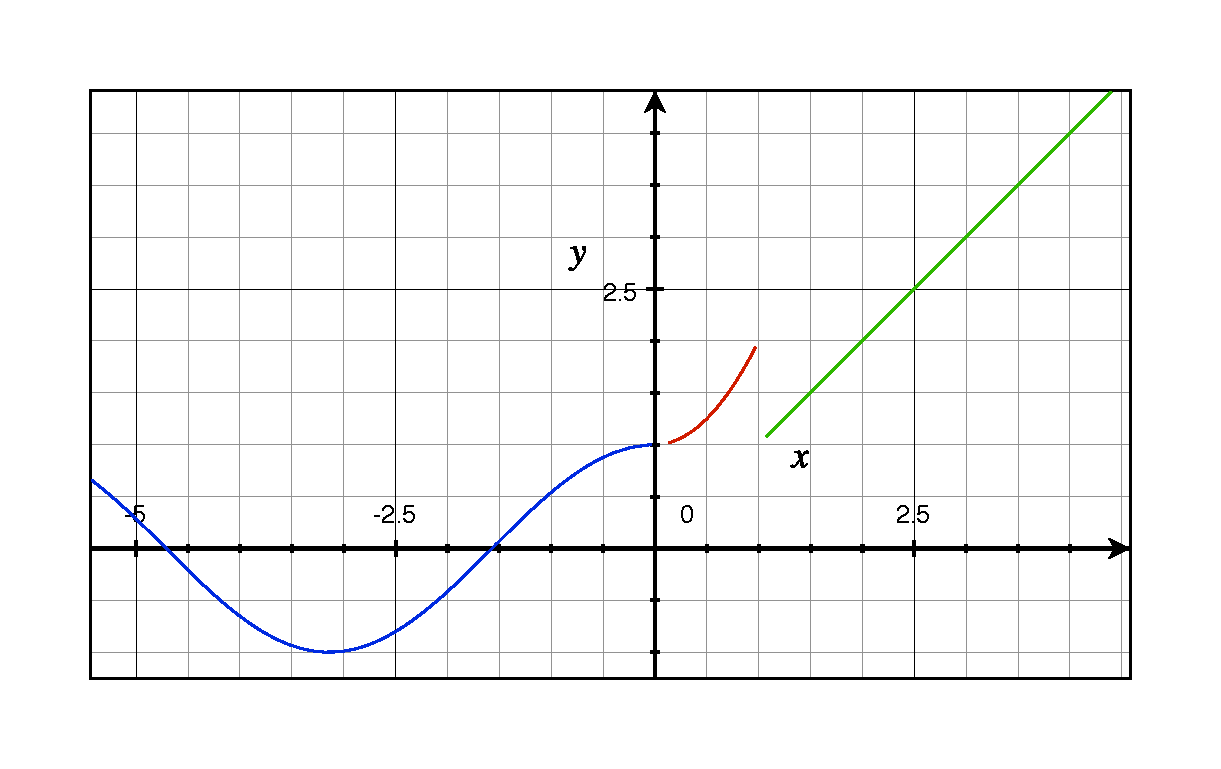
\includegraphics[width=450px,height=250px]{RG-Uni-Calculus-Reference_Work_1-04-1-5.eps}

\end{document}
